\chapter{Evaluatie}

\section{Preprocessing}

Deze stap bestaat uit drie fasen:
\begin{enumerate}
	\item Een translatie zorgt ervoor dat de \textit{Spine Base Joint} ($J_{sb}$) als oorsprong wordt genomen. Dit kan via een eenvoudige vectorbewerking 
	$$\begin{pmatrix}
	x' \\ y' \\ z'
	\end{pmatrix}
	= \begin{pmatrix}
	x \\ y \\ z
	\end{pmatrix}
	- \begin{pmatrix}
	x_0 \\ y_0 \\ z_0
	\end{pmatrix}$$
	
	waarbij $x_0, y_0$ en $z_0$ de drie-dimensionale coördinaten van $J_{sb}$ zijn. Deze transformatie zorgt ervoor dat de features \textbf{plaats-invariant} zijn. Een persoon kan zich nu eender waar bevinden in het camerabereik van de Kinect sensor.
	\item Een tweede fase is het schalen van de features. Dit kan ook eenvoudig berekend worden door de componenten van elke positievector van elk skelet joint te delen door een bepaalde norm $||n||$. Als norm wordt hier de lengte van de positievector van de \textit{Neck Joint} ($J_n)$ genomen en is gelijk aan
	$$||n|| = \sqrt{(J_{n_x})^2 + (J_{n_y})^2 + (J_{n_z})^2}$$
	Elke positievector kan dan genormeerd worden:
	$$
	\begin{pmatrix}
	x' \\ y' \\ z'
	\end{pmatrix}
	=				
	\begin{pmatrix}
	\frac{x}{||n||} \\ \frac{y}{||n||}  \\ \frac{z}{||n||} 
	\end{pmatrix}$$
	Men zou ook andere normen kunnen nemen. Figuur \todo{figuur} toont de impact van de keuze van verschillende normen.
	
	Deze schaaloperatie zorgt ervoor dat de features \textbf{schaal-invariant} zijn. Dit heeft vooral betrekking op personen met een kleiner en groter gestalte.
	\item Tot slot is er nog een rotatietransformatie die een nieuw soort coördinatensysteem introduceert. De features zijn nu ook \textbf{rotatie-invariant}.
\end{enumerate}
Figuur \ref{fig:skeleton_preprocessing} toont de invloed van de verschillende preprocessing fasen op de skeletdata.

\begin{figure}
	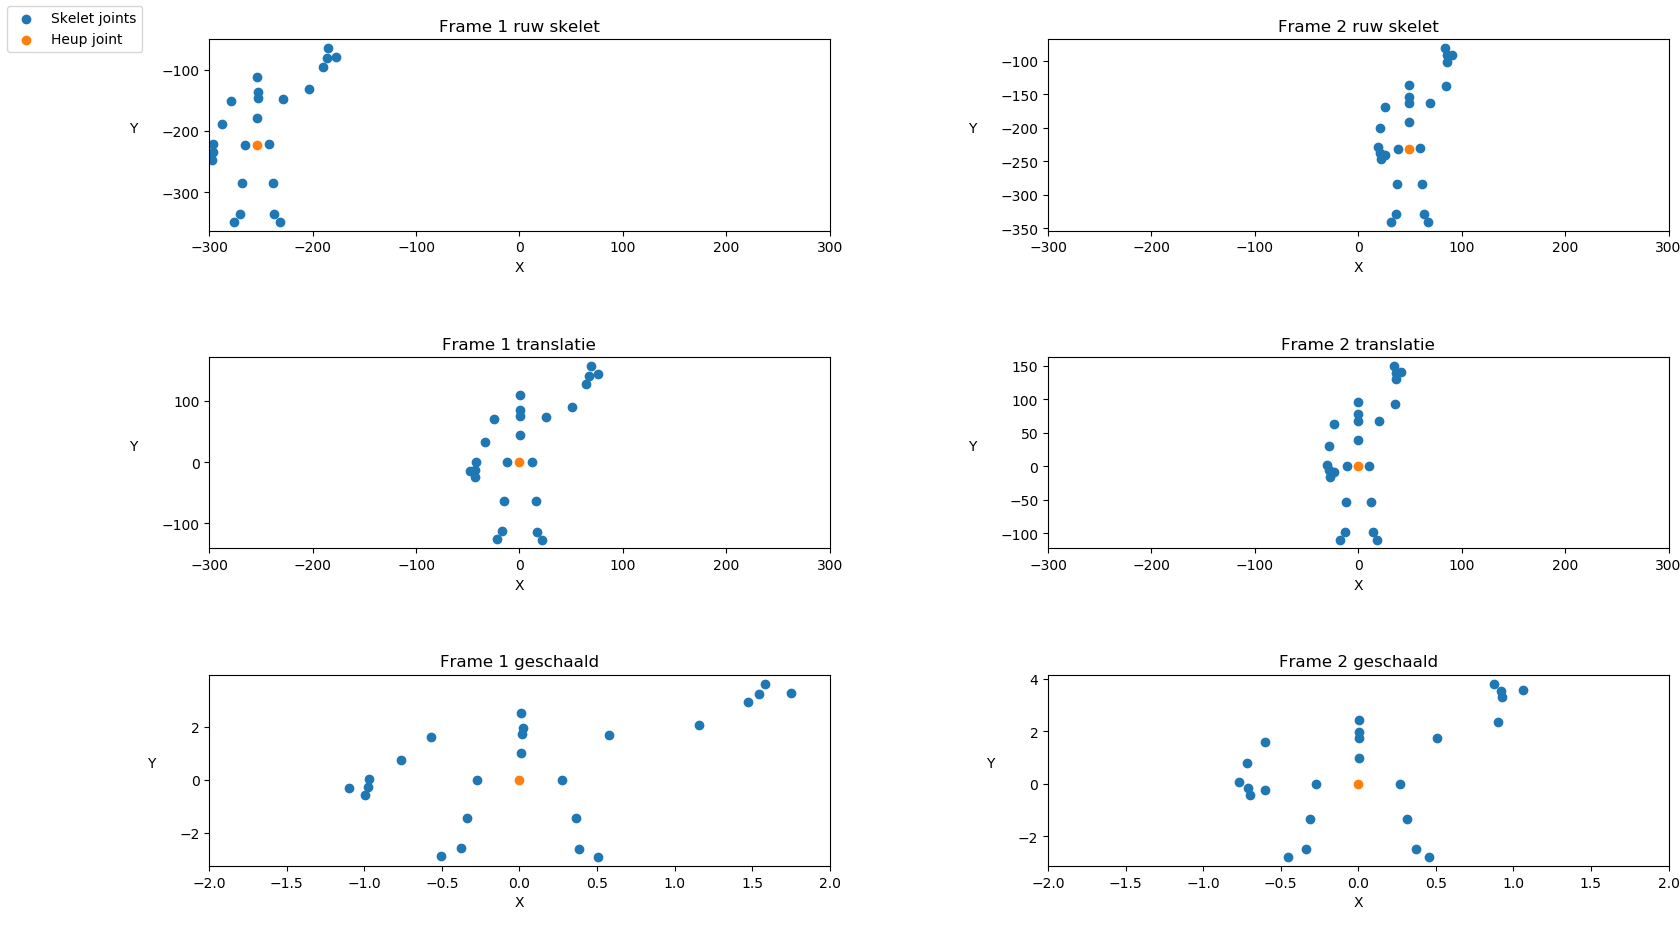
\includegraphics[width=\textwidth]{skeleton_preprocessing}
	\caption{De impact van de verschillende preprocessing fasen op twee gelijkaardige acties. Hierbij is de oranje joint de \textit{Spine Base joint}.}
	\label{fig:skeleton_preprocessing}
\end{figure}

\section{Classifiers}
\label{ch:evaluatie}
De gebruikte dataset bestaat uit $x$ acties. De \textit{classifier} kan voor elk frame één van deze acties toekennen. Om de classifier te evalueren zou er een $x \times x$ frequentietabel opgesteld kunnen worden waarbij zowel de rijen als de kolommen gelabeld worden met de namen van de acties. De \textit{classifier} heeft dan een correcte classificatie uitgevoerd als de rij en kolom overeenkomen. Een vereenvoudigd voorbeeld is te zien op tabel \ref{table:example_evaluation}
\begin{table}[ht]
	\centering
	\begin{tabular}{| c | ccc |}
		\hline
				& zwaaien & bukken & springen \\
				\hline
		zwaaien & \textbf{5} & 2 & 0 \\
		bukken & 1 & \textbf{11} & 4 \\
		springen & 0 & 0 & \textbf{4} \\
		\hline
		
	\end{tabular}
	\caption{Een voorbeeld van een $3 \times 3$ frequentietabel.}
	\label{table:example_evaluation}
\end{table}

Het is echter moeilijk om hieruit eenvoudig relevante statistieken te berekenen. Het is daarom interessanter om de informatie van die tabel te aggregeren voor elke klasse om een zogenaamde \textit{confusion matrix} te bekomen. Op die manier wordt een binair classificatiemodel gesimuleerd. Tabel \ref{table:example_evaluation_aggregate} toont een voorbeeld van een \textit{confusion matrix} voor de klasse \texttt{bukken}. 
\begin{table}[ht]
	\centering
	\begin{tabular}{| c | cc |}
		\hline
		& bukken & niet-bukken \\
		\hline
		bukken & 11 (TP) & 5 (FP) \\
		niet-bukken & 2 (FN) & 9 (TN)\\
		\hline
	\end{tabular}
	\caption{Een}
	\label{table:example_evaluation_aggregate}
\end{table}

Er zijn nu 4 statistieken beschikbaar. Ten eerste is er het aantal keer dat de \textit{classifier} de actie 'bukken' heeft herkend terwijl het effectief bukken was. Dit wordt een \gls{ac:tp} genoemd. Ten tweede is er het aantal keer dat de \textit{classifier} herkent heeft dat de persoon niet aan het bukken was en dat het werkelijk zo niet was. Dit wordt een \gls{ac:tn} genoemd. Deze twee statistieken tonen aan wanneer de \textit{classifier} een juiste classificatie heeft gedaan voor deze specifieke actie. De overige twee statistieken zijn de \gls{ac:fp} en \gls{ac:fn} die respectievelijk het aantal keer aanduiden dat het bukken is terwijl het niet zo was, en dat het niet bukken is terwijl het wel zo was. \todo{dit moet voor elke klasse uitgevoerd worden}

Aan de hand van deze vier waarden kunnen interessante statistieken berekent worden. Een populaire evaluatiemaat is het gebruik van de \textit{precision} en \textit{recall} statistieken, gedefinieerd als:

$$precision = \frac{TP}{TP + FP} \qquad recall = \frac{TP}{TP + FN}$$

De \textit{precision} bepaalt de kans dat een classificatie correct is als de classifier een positief resultaat geeft, terwijl de \textit{recall} de kans bepaalt dat de classificatie een positief exemplaar als positief zal classificeren).

% recall = the fraction of relevant documents that are succesfully retrieved
%			 given a positive example, will the classifier detect it?

% precision = the fraction of retrieved documents that are relevant to the query
%  	   	 	 given a positive prediction from the classifier, how likely is it to be correct?

\section{Segmentatie}



\section{Herkenning}